%--- Preamble ---------------------------------------------------------%
% Load LaTeX packages
\documentclass[12pt, xcolor=dvipsnames]{beamer}
\usepackage[absolute, overlay]{textpos}                           % supports floating text in any location
\usepackage[utf8]{inputenc}
\usepackage{tikz}
\usepackage{csquotes,xpatch}% recommended
%\usepackage[english]{babel}
%\usepackage[american]{babel}
\usepackage[brazil]{babel}
\usepackage{hyperref}
\usepackage{graphicx}
\usepackage{tabularx}
\usepackage{booktabs}
\usetikzlibrary{shapes}
\usetikzlibrary{arrows}
\usetikzlibrary{positioning}
\usetikzlibrary{calc}

% Customize theme attributes
\useoutertheme{infolines}					                     % adds 3 box footer
\usetheme[height=7mm]{Rochester} 				                 % choose theme
\setbeamertemplate{blocks}[rounded][shadow=true] 		         % rounded theorem box with shadow
\setbeamertemplate{caption}[numbered]                             % enable counting of tables/figures

% Define template colors
\definecolor{QPblue}{RGB}{0,25,100}                               % define QP blue using RGB code
\definecolor{QPgreen}{RGB}{0,153,110}                             % define QP green using RGB code
\setbeamercolor{title}{fg=white, bg=QPblue}                       % define title page box color
\setbeamercolor{frametitle}{fg=white, bg=QPblue}                  % define frame title color
\setbeamercolor{normal text}{fg=black}                            % define standard font color
\setbeamercolor{author in head/foot}{fg=QPblue, bg=QPblue!75}    % define infoline 1st box color
\setbeamercolor{title in head/foot}{fg=QPblue, bg=QPblue!60}     % define info line 2nd box color
\setbeamercolor{date in head/foot}{fg=QPblue, bg=QPblue!30}	  % define infoline 3rd box color
\setbeamercolor{block title}{fg=QPblue!50!QPgreen, bg=QPblue!30} % define theorem box title color
\setbeamercolor{block body}{fg=QPblue!50!QPgreen, bg=gray!10}	 % define theorem box body color
\setbeamercolor{local structure}{fg=QPblue!75}		           % define bullet and enumerate list colors

% Define global environments
\newenvironment{reference}[2]{                                    % define environment for footnotes
  \begin{textblock*}{\textwidth}(#1, #2)
      \tiny\it\bgroup\color{red!70!QPblue}}{\egroup\end{textblock*}}

% Define title page logo and project metadata
\titlegraphic{
\includegraphics[width=3cm]{UNINOVE_LOGO.JPG}\hspace*{0cm}~
}

\title{Como avaliar evidências científicas?}
\subtitle{Ateliê da Linha de Pesquisa de Estratégia}
\author{Jose Storopoli}
\institute[Programa de Pós-Graduação em Administração - Mestrado e Doutorado]{
   \textcolor{QPblue!75}{Universidade Nove de Julho \\
   UNINOVE \\
   São Paulo \\
   Brasil \\ [1ex]
   \texttt{josees@uni9.pro.br}}
}
\date{Maio 2022}

\begin{document}

%--- Title Page -------------------------------------------------------%

\begin{frame}[plain]
  \titlepage
  \begin{reference}{4mm}{90mm}
    Slides e Código Julia em \href{https://github.com/storopoli/evidencias-cientificas}{\texttt{storopoli/evidencias-cientificas}}
  \end{reference}
\end{frame}

%--- Slide 1 ----------------------------------------------------------%

\begin{frame}{Cargo Cult Science}
  \begin{columns}
    \begin{column}{0.45\textwidth}
      \begin{figure}[p]
        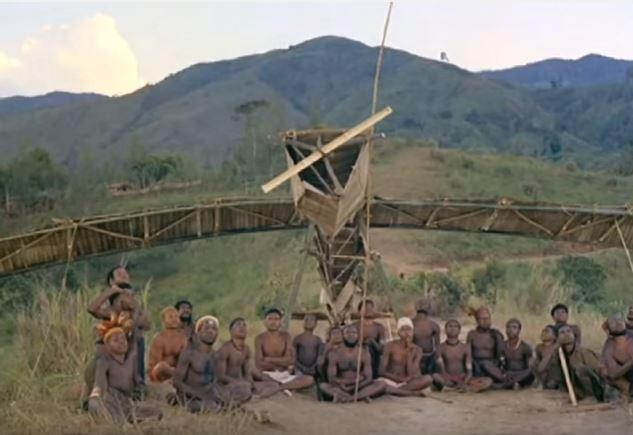
\includegraphics[width=6cm]{images/cargo_cult.png}<2->
    \end{figure}
    \end{column}
    \begin{column}{0.45\textwidth}
      \begin{itemize}
        \item<3-> Melanésia (Oceania) durante Segunda Guerra Mundial
        \item<4-> Culturas isoladas em ilhas entram em contato com forças aliadas
        \item<5-> Depois da guerra os soldados foram embora com seus aviões e cargas
      \end{itemize}
    \end{column}
  \end{columns}
  \begin{reference}{4mm}{85mm}
    Feynman, R. (1974). Cargo cult science. Caltech commencement address.
  \end{reference}
\end{frame}

%--- Slide 2 ----------------------------------------------------------%

\begin{frame}{O que é Ciência do Culto à Carga?}
  \begin{itemize}
    \item<2-> Os nativos sentindo falta dos suprimentos começaram a imitar o comportamento dos soldados
    \item<3-> Assim esperando que isso faria voltar os aviões \uncover<4->{... mas eles não voltaram}
    \item<5-> \textbf{Ciência do Culto à Carga} é exatamente isso:
    \begin{itemize}
      \item<6-> Tem "citações"
      \item<7-> Tem "metodologia"
      \item<8-> Tem até "tabelas estatísticas"  \uncover<9->{... e $p$-valores!}
      \item<10-> \textbf{Pseudociência!}
    \end{itemize}
  \end{itemize}
  \begin{reference}{4mm}{85mm}
    Feynman, R. (1974). Cargo cult science. Caltech commencement address.
  \end{reference}
\end{frame}

%--- Slide 3 ----------------------------------------------------------%

\begin{frame}{Cargo Cult Statistics}
  \begin{itemize}
      \item<2-> A mímica ritualística de estatísticas, em vez da prática conscienciosa
      \item<3-> Isso se tornou a norma em muitas disciplinas, reforçado e estimulado:
      \begin{itemize}
        \item<4-> educação estatística
        \item<5-> software estatístico
        \item<6-> políticas editoriais
      \end{itemize}
      \item<7-> Ciência deveria ser \textbf{"Show me"} e não \textbf{"Trust me"}
    \end{itemize}
  \begin{reference}{4mm}{85mm}
    Stark, P. B., \& Saltelli, A. (2018). Cargo-cult statistics and scientific crisis. Significance, 15(4), 40–43.
    \url{https://doi.org/10.1111/j.1740-9713.2018.01174.x}
  \end{reference}
\end{frame}

%--- Slide 4 ----------------------------------------------------------%

\begin{frame}{Cargo Cult Statistics}
  \begin{itemize}
      \item<2-> Muitas aplicações de estatística são \textbf{Culto à Carga}:
      \begin{itemize}
        \item<3-> estimar modelos
        \item<3-> computar $p$-valores ou intervalos de confiança
        \item<3-> simular densidades posteriores
        \item<3-> termos estatísticos
      \end{itemize}
      \item<4-> Porém pouco\footnote<4->{às vezes nenhum...} \textbf{entendimento} sobre:
      \begin{itemize}
        \item<5-> pressupostos das técnica
        \item<5-> relevância dos valores
        \item<5-> significado da terminologia
      \end{itemize}
      \item<6-> Isso rebaixa as estatísticas de uma \textbf{forma de pensar sobre as evidências e evitar a auto-ilusão}
      para uma \textbf{"bênção" formal de alegações}.
    \end{itemize}
  \begin{reference}{4mm}{80mm}
    Stark, P. B., \& Saltelli, A. (2018). Cargo-cult statistics and scientific crisis. Significance, 15(4), 40–43.
    \url{https://doi.org/10.1111/j.1740-9713.2018.01174.x}
  \end{reference}
\end{frame}


%--- Slide 5 ----------------------------------------------------------%

\begin{frame}{Cargo Cult Statistics -- Frequentista vs Bayesiana}
  \begin{columns}[T]

    \begin{column}{0.45\textwidth}
      {\Large \textbf{Frequentista}}
      \begin{itemize}
        \item $p$-valores
      \end{itemize}
    \end{column}

    \begin{column}{0.45\textwidth}
      {\Large \textbf{Bayesiana}}
      \begin{itemize}
        \item \textit{Priors}
      \end{itemize}
    \end{column}
  \end{columns}

  ~\\[2ex]
  \uncover<2->{Estatística \textbf{frequentista} é sobre o que você faria se tivesse um \textbf{modelo}, e
  estatística \textbf{Bayesiana} e sobre o que você faria se tivesse uma \textbf{\textit{prior}}.}

  \begin{reference}{4mm}{85mm}
    Stark, P. B., \& Saltelli, A. (2018). Cargo-cult statistics and scientific crisis. Significance, 15(4), 40–43.
    \url{https://doi.org/10.1111/j.1740-9713.2018.01174.x}
  \end{reference}
\end{frame}

%--- Slide 6 ----------------------------------------------------------%

\begin{frame}{Maioria dos achados publicados são \textbf{falsos}}
  \begin{itemize}
    \item<2-> Mais uma vez nosso amigo $p$-valor
    \item<3-> Se adotarmos $p < 0.05$, 1 a cada 20 estudos serão "falsos positivos"
    \item<4-> Se há um "viés de publicação" para somente aceitar/publicar achados positivos
    \item<5-> Logo: \textbf{a proporção de 5\% acaba sendo exarcebada}
  \end{itemize}

  ~\\[2ex]
  \centering
  \uncover<6->{\alert{Achados Falsos} e \alert{Crise de Replicabilidade}}

  \begin{reference}{4mm}{85mm}
    Ioannidis, J. P. A. (2005). Why most published research findings are false. PLoS Medicine, 2(8), e124.
  \end{reference}
\end{frame}

%--- Slide 7 ----------------------------------------------------------%

\begin{frame}{Moderação}
  \begin{figure}[H]
    \begin{center}
      \begin{tikzpicture}[shorten >=1pt,node distance=5cm,auto]%,on grid
        \tikzstyle{every node}=[thick, draw, ellipse, minimum size=1.5cm, align=center]
        \node (densidade) {densidade\\ demográfica};
        \node[right=of densidade] (transito) {trânsito};
        \node[above right=2.95cm of densidade] (chuva) {chuva};
        \path [->,draw,thick] (chuva) -- ($ (densidade) !.5! (transito) $);
        \path [->,draw,thick] (densidade) -- (transito);
      \end{tikzpicture}
    \end{center}
  \end{figure}
\end{frame}

%--- Slide 8 ----------------------------------------------------------%

\begin{frame}{Moderação}
  \centering
    \begin{tabular}{lr}
\toprule
                              & \multicolumn{1}{c}{Trânsito} \\ 
\cmidrule(lr){2-2} 
                              &                          (1) \\ 
\midrule
(Constante)                   &                        0.000 \\ 
                              &                      (0.000) \\ 
Densidade Demográfica         &                     0.827*** \\ 
                              &                      (0.003) \\ 
Chuva                         &                        0.002 \\ 
                              &                      (0.002) \\ 
Densidade Demográfica * Chuva &                     0.223*** \\ 
                              &                      (0.003) \\ 
\midrule
$R^2$                         &                        0.996 \\ 
\bottomrule
\end{tabular}

\end{frame}

%--- Slide 9 ----------------------------------------------------------%

\begin{frame}{Moderação}
  \begin{figure}[H]
    \begin{center}
      \begin{tikzpicture}[shorten >=1pt,node distance=5cm,auto]%,on grid
        \tikzstyle{every node}=[thick, draw, ellipse, minimum size=1.5cm, align=center]
        \node (distancia) {distância\\ solar};
        \node[right=of distancia] (temperatura) {temperatura};
        \node[above right=2.85cm of distancia] (reflex) {coeficiente\\ de reflexão};
        \path [->,draw,thick] (reflex) -- ($ (distancia) !.5! (temperatura) $);
        \path [->,draw,thick] (distancia) -- (temperatura);
      \end{tikzpicture}
    \end{center}
  \end{figure}
\end{frame}

%--- Slide 10 ----------------------------------------------------------%

\begin{frame}{Moderação}
  \centering
    \begin{tabular}{lr}
\toprule
                                          & \multicolumn{1}{c}{Temperatura} \\ 
\cmidrule(lr){2-2} 
                                          &                             (1) \\ 
\midrule
(Constante)                               &                           0.000 \\ 
                                          &                         (0.000) \\ 
Distância Solar                           &                       -0.845*** \\ 
                                          &                         (0.032) \\ 
Coeficiente de Reflexão                   &                          -0.007 \\ 
                                          &                         (0.023) \\ 
Distância Solar * Coeficiente de Reflexão &                        0.225*** \\ 
                                          &                         (0.032) \\ 
\midrule
$R^2$                                     &                           0.496 \\ 
\bottomrule
\end{tabular}

\end{frame}

%--- End -------------------------------------------------------------%
\end{document}
